\documentclass[../main.tex]{subfiles}
\begin{document}
\subsubsection{Different timescales: rate-induced (R-)tipping}\label{subsubsec3.1.2}
The modelling of critical transitions in the fast-slow formulation also introduces an additional mechanism driving the tipping in which the ramping of the parameter is itself the cause of sudden regime shifts in the dynamics. 
In \cite{Ashwin12} the rate of change of $\mu$ is shown to cause, for some specific critical values, sudden regime shifts in the dynamics of a fast-slow system that does not feature a deterministic bifurcation, otherwise known as R-tipping. 
\begin{definition}[]\label{def3.2}
        Let $x\in \mathbb{R}^{n}$ be a state variable, $\mu\in \mathbb{R}$ a time-changing parameter, $R>0$ a constant and $M$ a fixed, stable and invertible linear operator then the linearised system
        \begin{equation*}
             \newprime{x}(t)=M(x-x^{*}(\mu)),
        \end{equation*}
        is said to be (adiabatically) tracking the stable equilibria $x_{\text{eq}}(\mu)$ if $\forall t\;|x(t)-x_{\text{eq}}(\mu(t))|<R$ and viceversa it tips beyond the equilibria if $\exists t_{0}\;\text{s.t.}\;|x(t_0)-x_{\text{eq}}(\mu(t_0))|=R$. 
\end{definition}
The so-called tipping radius $R$ is identified by constructing the condition upon which a fast-slow system fails to track the (slow) drift of the attractor
To study the dependence of the tipping event from the rate of change of the time-varying parameter we formally introduce the drift of the stable equilibria
\begin{equation*}
        r(t):=\frac{d}{dt}(x_{\text{eq}}(\mu(t))) = \frac{dx_{\text{eq}}}{d\mu}\frac{d\mu}{dt} = \varepsilon \frac{dx_{\text{eq}}}{dt}\,.
\end{equation*}
With these quantities defined we are ready to define a criterion for R-tipping for systems with steady drift.
\begin{theorem}[label=thm3.2]{}{}
Let \eqref{eq3.1} be a system with tipping radius $R>0$ and $r(t)=r>0$ is constant (i.e. steady drift of the parameter), then 
\begin{equation*}
          ||M||^{-1}|r|>R
\end{equation*}
is a sufficient condition for R-tipping to occur.
\end{theorem}
\begin{proof}
     Given an initial condition $x(0)=x_{0}$ the general solution of \eqref{eq3.1} is
     \begin{equation*}
         x(t) = e^{Mt}x_{0}+\int_{s=0}^{t}e^{M(t-s)}M\,x_{\text{eq}}(\mu(s))\,ds = - \int_{u=0}^{\infty}e^{Mu}M\,x_{\text{eq}}(\mu(t-u))\,du\,,
     \end{equation*}
     where the dependence on the initial condition is dropped from the second integral by assuming an arbitrarly long past while setting $u:=t-s$. Integrating by parts the general solution gives us
     \begin{equation*}
             x(t) = -[e^{Mu}x_{\text{eq}}(\mu(t-u))]_{0}^{\infty} - \int_{0}^{\infty}e^{Mu}\frac{d}{dt}(x_{\text{eq}}(\mu(t-u)))\,du\:\Rightarrow\: x(t) - x_{\text{eq}}(\mu(t)) = -\int_{0}^{\infty}e^{Mu}r(\mu(t-u))\,du\,,
     \end{equation*}
     where the (exponential) stability of the linear operator $(|e^{Mt}\to0|\;\text{as}\; t\to \infty)$ has been used. We integrate by parts again and obtain 
     \begin{equation*}
         x(t) - x_{\text{eq}}(\mu(t)) = M^{-1}r(\mu(t-u))-\int_{0}^{\infty}e^{Mu}M^{-1}\,\newprime{r}(\mu(t-u))\,du\,.
     \end{equation*}
     Assuming now steady drift the above simplifies to
     \begin{equation*}
         x(t) - x_{\text{eq}}(\mu(t)) = M^{-1}r\;\Rightarrow\;|x(t) - x_{\text{eq}}(\mu(t))| = |M^{-1}r|\,.
     \end{equation*}
     By choosing the matrix norm for the linear operator $||M||=\text{sup}_{v\neq0}\frac{|Mv|}{|v|}$ then it trivially follows
     \begin{equation*}
         ||M||^{-1}|r|\leq|M^{-1}r|\leq||M^{-1}|||r|\,.
     \end{equation*}
     We now recall from Definition \ref{def3.2} the condition for R-tipping which gives us the sufficient condition $||M||^{-1}|r|>R$ for the solution to slip off the stable equilibria thereby causing the rate-induced critical transition.
\end{proof}
This result allows us to generalise the analysis to systems that have no known deterministic bifurcations therefore dropping the additional constraint of restricting ourselves to problems that can be recast in a normal form.
\begin{example}[label=ex3.2]{}{}
As an example we consider the following $2-$dimensional model of compost-bomb instability \cite{Wieczorek11} in the slow timescale
\begin{equation*}
        \begin{cases}
            \varepsilon \newprime{x} = y + \mu + x(x-1)\,, \\
            \newprime{y} = - x - x^2 - x^{3} - x^{4} - x^{5}\,,
        \end{cases}
\end{equation*}
with steady (linear) ramping of the parameter $\mu\in \mathbb{R}$.
The system has one stable equilibrium at $(0,-\mu)$ and in the singular limit we are able to derive the critical manifold 
\begin{equation*}
            C=\{(x,y)\in \mathbb{R}^{2}\;:\;y=-\mu-x(x-1)\}\,,
\end{equation*}
with attracting $C^{(a)}=\{C\cap\{x<\frac{1}{2}\}\}$ and repelling $C^{(r)}=\{C\cap\{x>\frac{1}{2}\}\}$ submanifolds separated by a saddle line which is tangent to $C$ along $x=\frac{1}{2}$. Note that the distance along $x$ between the stable equilibrium and the fold of the critical manifold is exactly $\frac{1}{2}=R$ which will thus provide us the tipping radius for our system.
We now differentiate the critical manifold w.r.t. the slow timescale to obtain
\begin{align}
        0 =&\;\dot{x} + \dot{\mu} + \frac{d}{d\tau}(x^{2}-x) = f_{2}(x, y) + r + \dot{x}(2x-1)\;\Rightarrow \nonumber \\
        \Rightarrow&\;\dot{x}=-\frac{f_{2}(x, y)+r}{2x-1} \,, \label{eq3.4}
\end{align}
where we have $f_{2}(x, y):=\dot{y}=- x - x^{2} - x^{3} - x^{4} - x^{5} = -\sum_{n=1}^{5}x^{\,n}$ for the slow dynamics as well as the definition for the drif $\dot{\mu} =: r$.
We immediately realise that \eqref{eq3.4} is singular along the fold of the critical manifold therefore, by recalling that $\tau = \epsilon t\;\Rightarrow\;\frac{dt}{d\tau}=\epsilon^{-1}$, we shift the temporal framework onto the fast timescale $t$ obtaining
\begin{equation}\label{eq3.5}
   \begin{cases}
      \newprime{x} = r - \sum_{n=1}^{5}x^{n}  \,, \\
      \newprime{\mu} = -r(2x-1) \,, 
   \end{cases}
\end{equation}
The equilibria for \eqref{eq3.5} will finally give us the (parametrised) invariant set of $x$ points to which trajectories starting within the attracting submanifolds will converge to
\begin{equation*}
        M(r) = \{(x, y)\in \mathbb{R}^{2}\;:\;\sum_{n=1}^{5}x^{n}=r\}
\end{equation*}
To find the critical value $r_{c}$ for the drift of the parameter that causes the state to tip and slip off the critical manifold we only need to substitute the value for the tipping radius previously derived in $M(r)$ which thus gives us $r_{c}\approx 0.9687$.
We conclude that drift values $r>r_{c}$ will move the invariant set over and across the fold of the critical manifold meaning that even those trajectories that start within $C^{(a)}$ will slip off the stable equilibria and tip in a rate-induced critical transition.
\end{example}
\begin{example_continued}
\begin{figure}[H]
    \centering 
    \begin{subfigure}[b]{0.485\textwidth}
        \centering 
        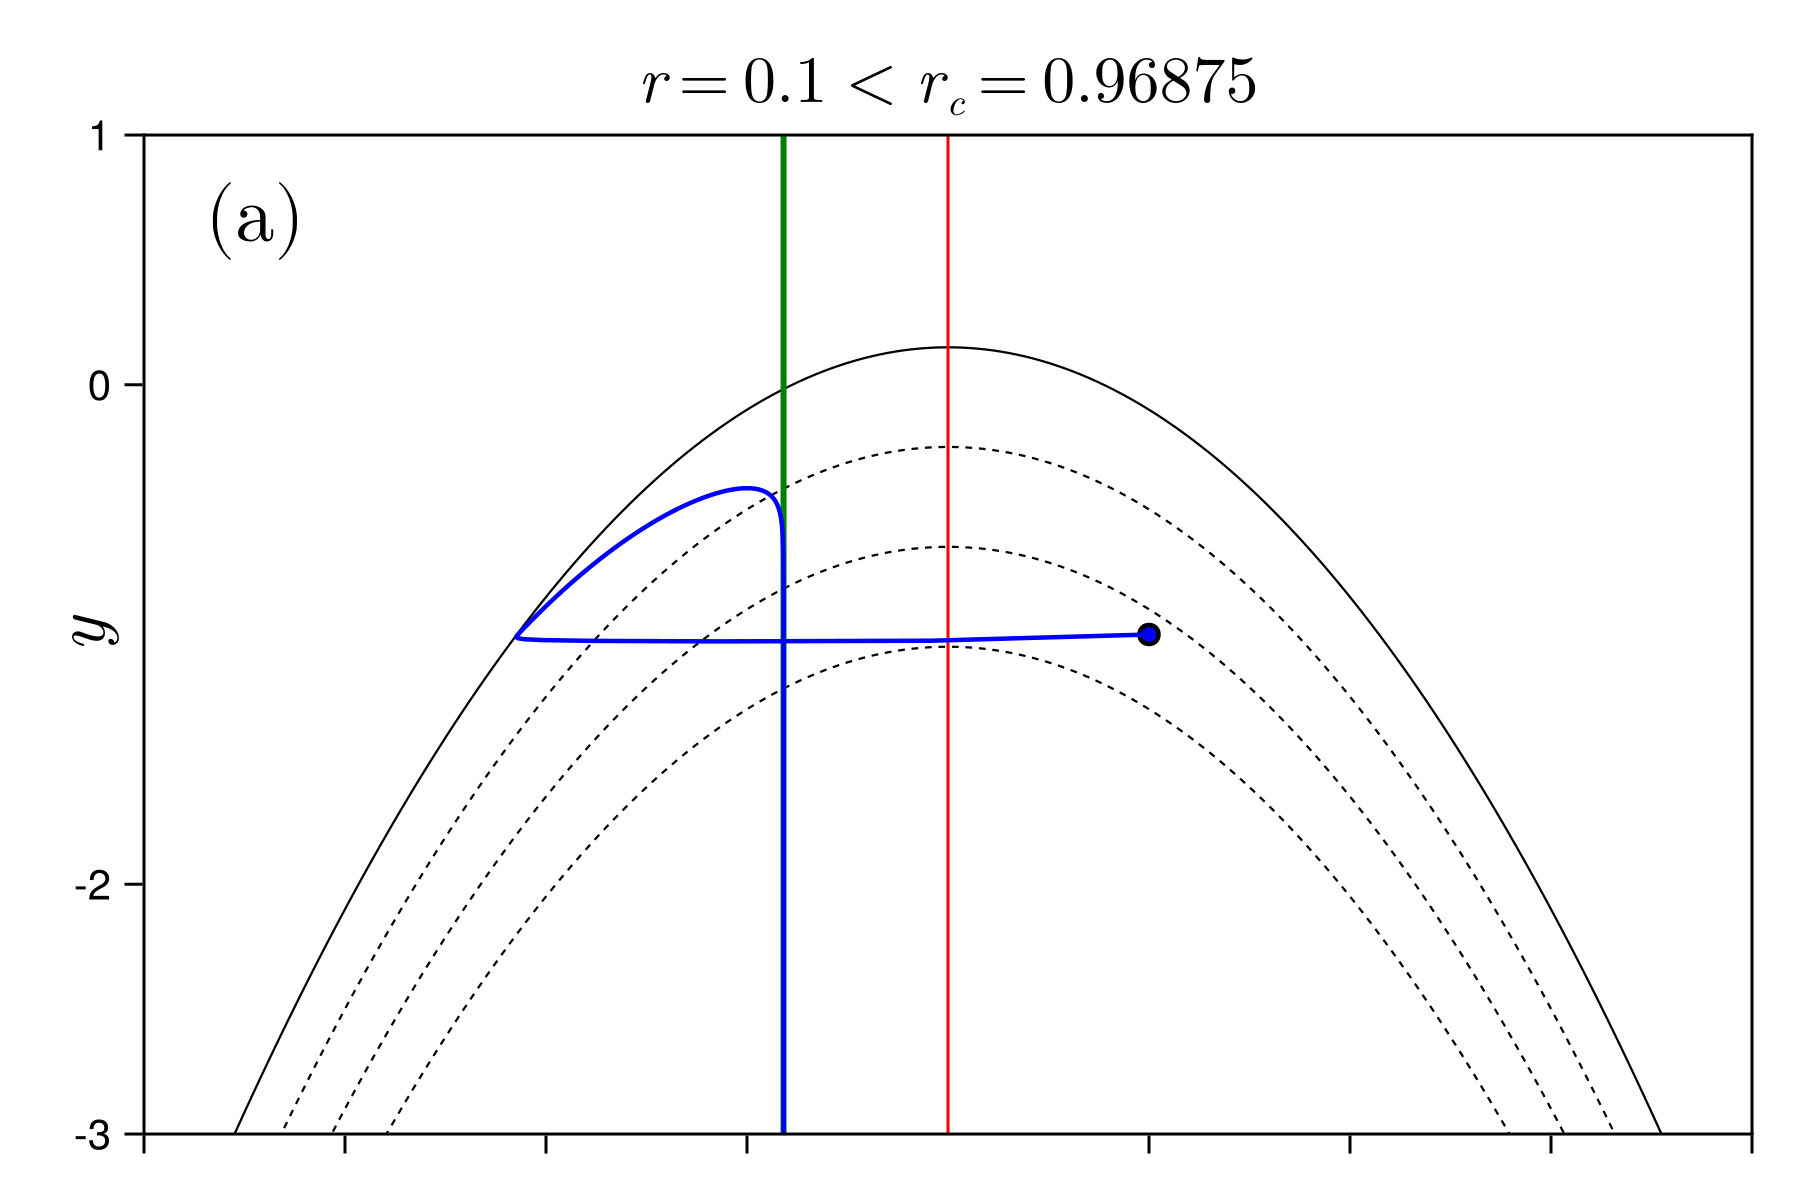
\includegraphics[keepaspectratio, width = \linewidth]{../figures/fig3.2.1.png}
        \label{fig3.2.1}
    \end{subfigure}
    \hfill 
    \begin{subfigure}[b]{0.485\textwidth}
        \centering 
        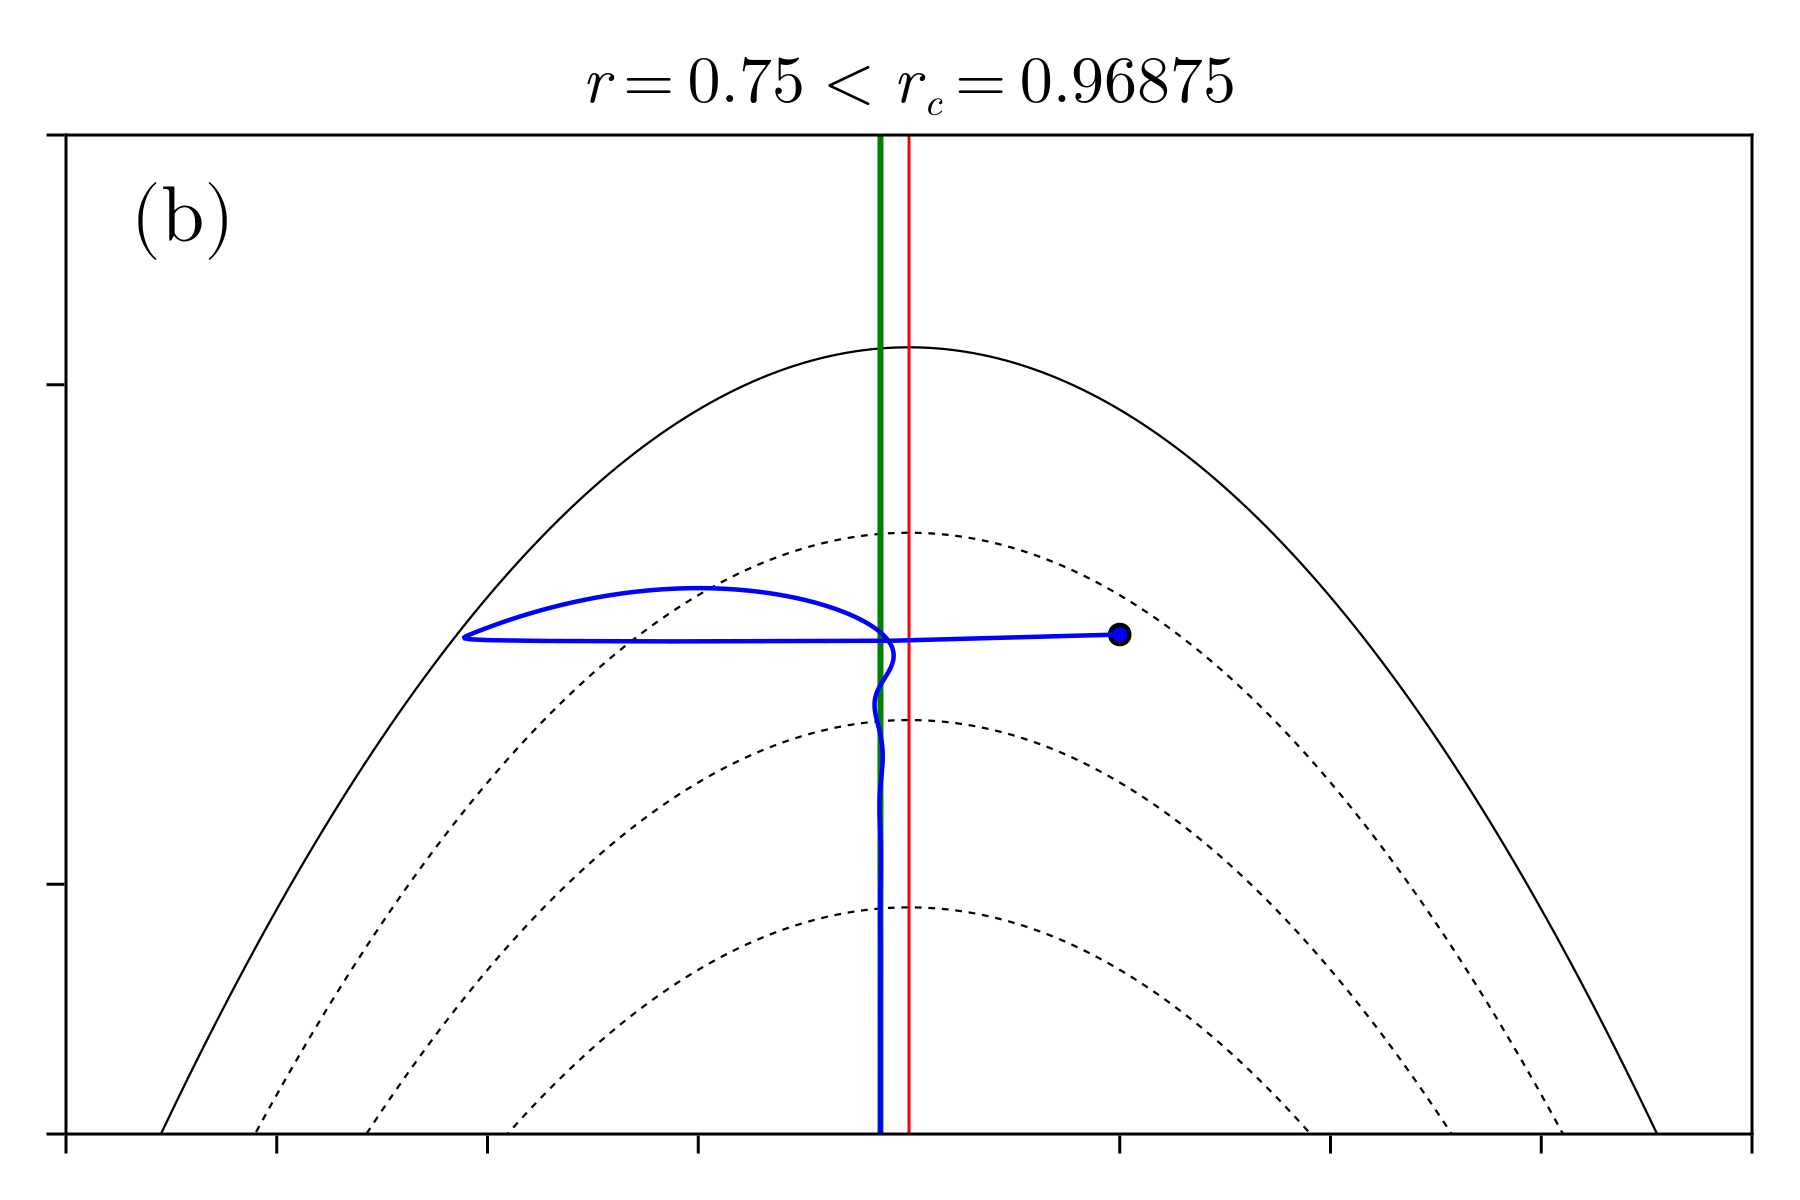
\includegraphics[keepaspectratio, width = \linewidth]{../figures/fig3.2.2.png}
        \label{fig3.2.2}
    \end{subfigure}


    \begin{subfigure}[b]{0.485\textwidth}
        \centering 
        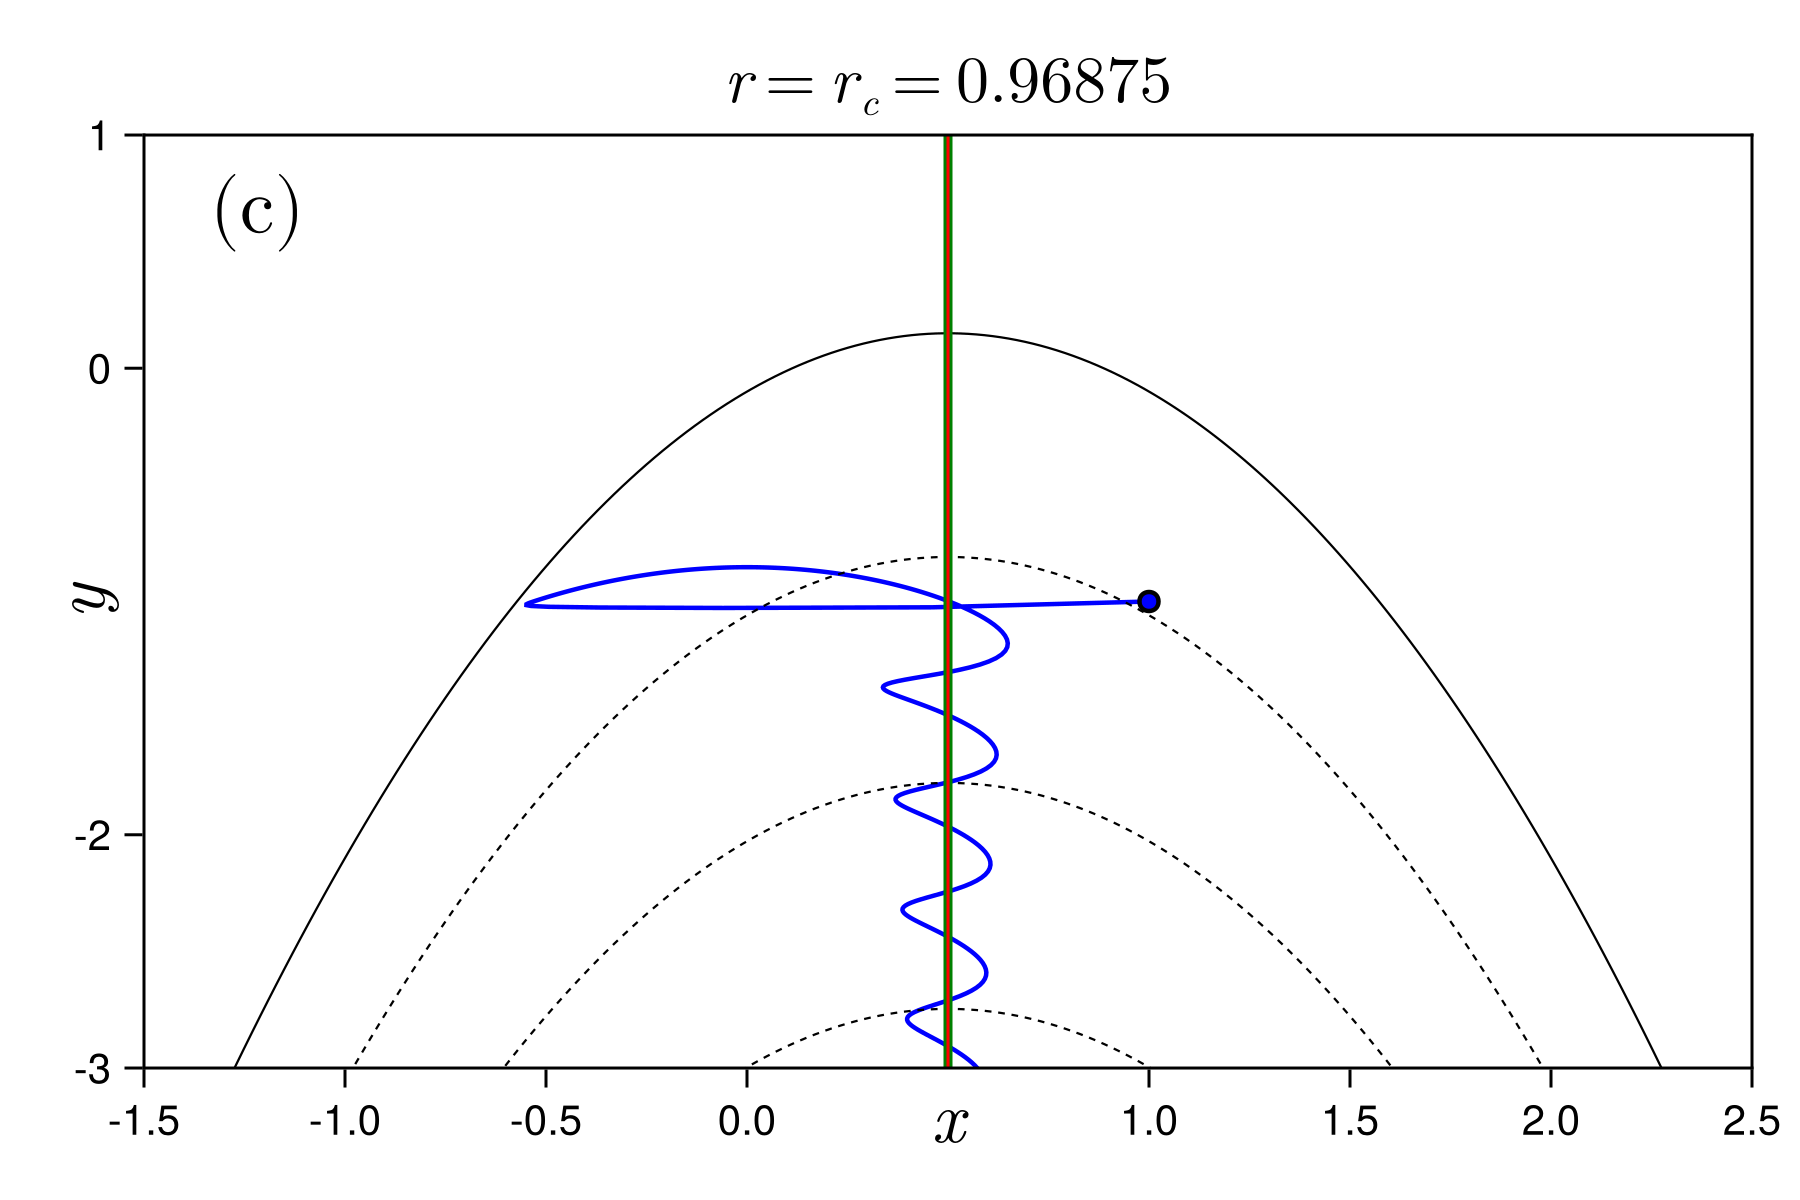
\includegraphics[keepaspectratio, width = \linewidth]{../figures/fig3.2.3.png}
        \label{fig3.2.3}
    \end{subfigure}
    \hfill
    \begin{subfigure}[b]{0.485\textwidth}
        \centering 
        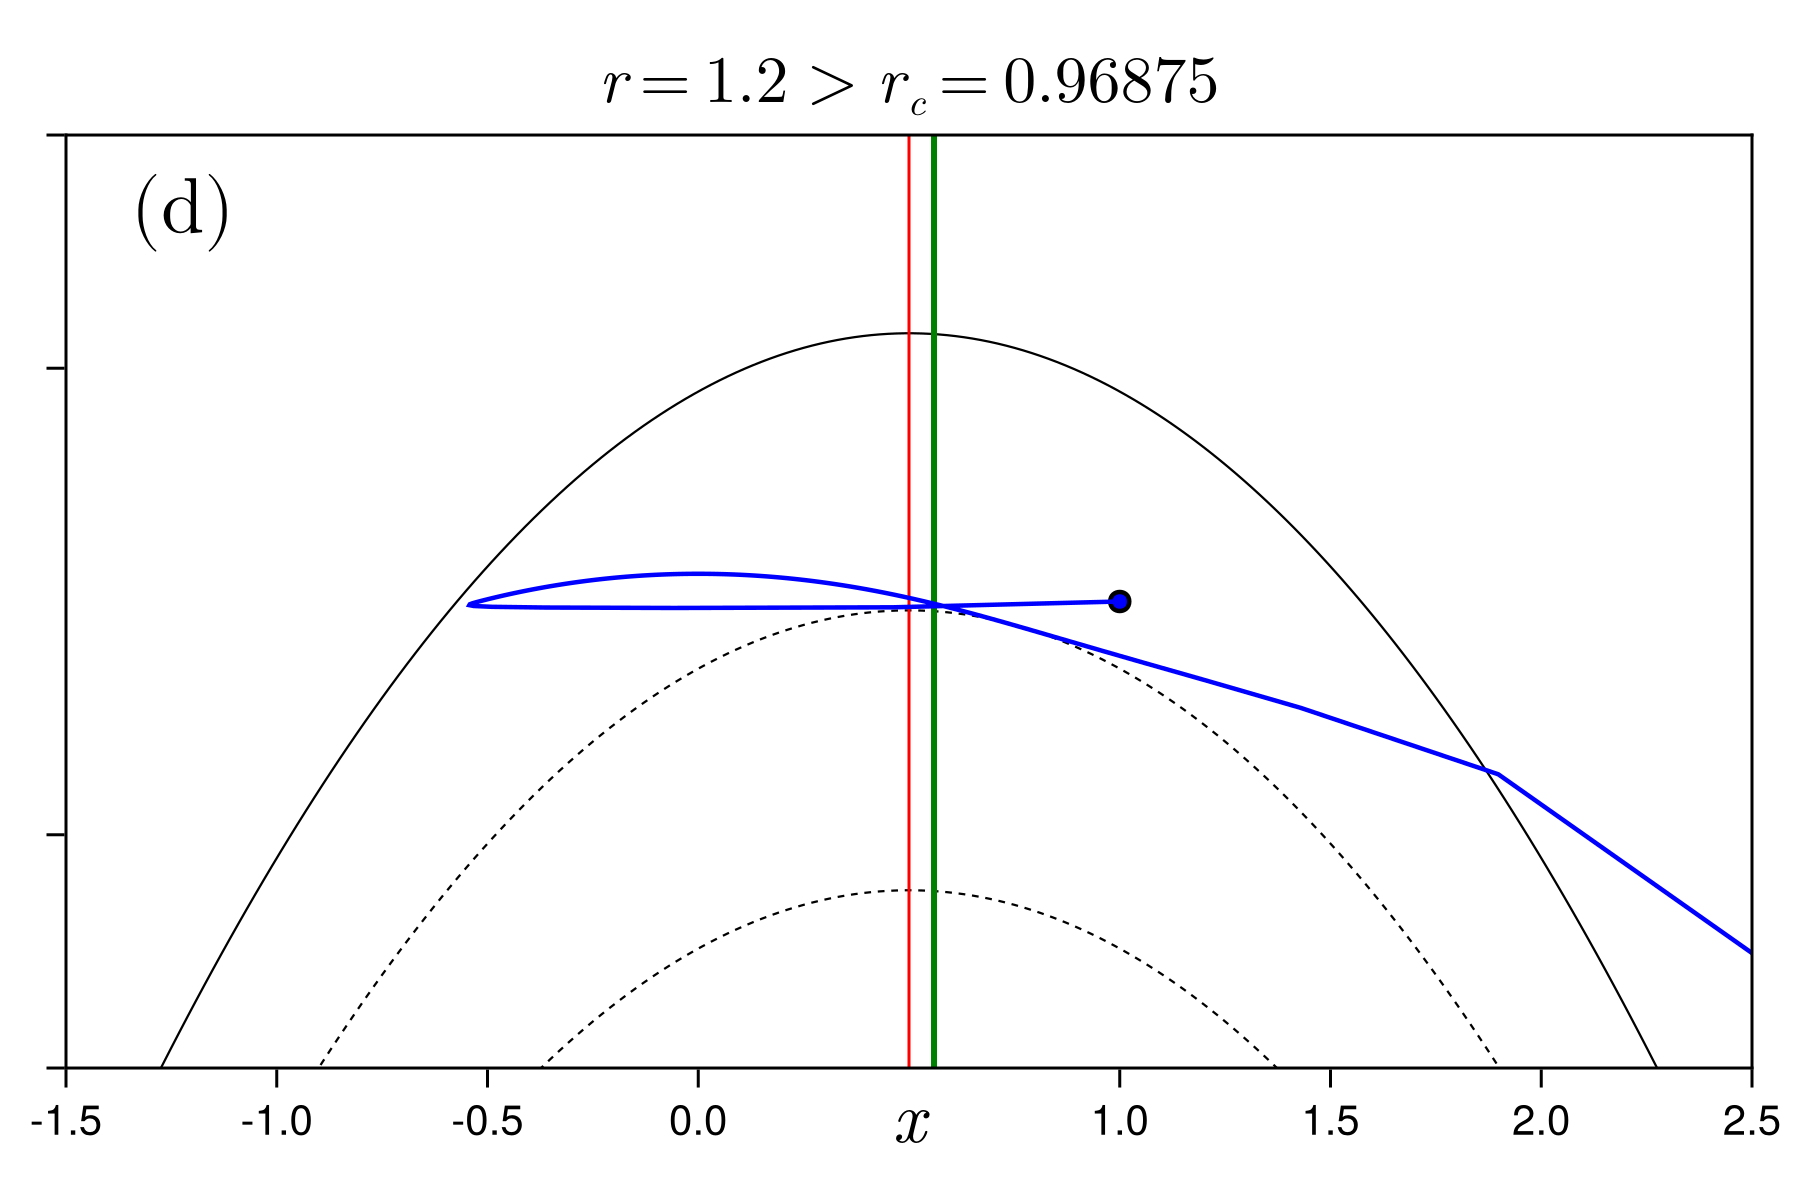
\includegraphics[keepaspectratio, width = \linewidth]{../figures/fig3.2.4.png}
        \label{fig3.2.4}
    \end{subfigure}
    \caption{Forward-time trajectories (blue curves) of the compost-bomb fast-slow system propagated from the IC $(1,-1)$ (blue dots) located in the inner part of the attracting submanifold $C^{(a)}$ with timescale separation value $\varepsilon = 2\cdot10^{-2}$ and parameter $\mu$ varied linearly in $[0,2]$ at different rates $r(t)$.
            Notice how as we keep increasing the drift of the parameter while keeping it below the critical value (a)$\sim$(b) the invariant set (solid red line) moves closer to the fold of the critical manifold (here depicted as the solid black curve for the initial parameter value of $\mu=0.1$ and as dashed black curves at increasing parameter values) but never crosses it, allowing the trajectories to eventually settle on the invariant set (solid green lines) meaning that they will remain close (within tipping radius distance) to the stable equilibrium. 
    For a drift corresponding to the critical value $r_{c}$ (c) we notice large oscillations while the trajectories try to settle along the invariant set which has now moved over and overlapping with the saddle.
Finally as we keep increasing the drift over the critical value (d) we clearly see that now the invariant line as crossed over the fold and thus the trajectories are now unable to track the stable equilibrium thereby slipping off the critical manifold.}
    \label{fig3.2}
\end{figure} 
\end{example_continued}
As mentioned in the description of Figure \ref{fig3.1} the non-stationarity of the parameter implies a delay in the tipping event. 
As such a natural question arises in how this delay reflects in the detection of EWS of R-tipping events. 
In 2016 Ritchie and colleagues \cite{Ritchie16} observed that an increase in variance and autocorrelation also feature the same delay w.r.t. the critical parameter drift value and analytically characterised it for a saddle-node normal form.
6 years later in 2023 Ritchie et al. \cite{Ritchie23} revisited this concept for more complex settings of predator-prey ecological systems and the possible collapse of the Atlantic meridional overturning circulation (AMOC), both with non-linear ramps of the forcing parameter.
The same climate model was used 2 years prior \cite{Lohmann21} to conclude how R-tipping could in principle lead to a cascading effect of tipping points predicted by an increase in variance and autocorrelation.
\end{document}
